\section{第十章\quad 蒸汽动力装置循环}

%1、2、3 ppt 全部

\pt{蒸汽动力装置}：锅炉/过热器吸热，汽轮机膨胀作功，冷凝器定压放热凝结，水泵升压送回锅炉。冷凝器不能取消：它排热并维持低背压，使循环闭合且汽轮机能充分膨胀。

\pt{水蒸气卡诺循环不采用}：温限小；膨胀末端干度 $x$ 太小，湿蒸汽冲蚀叶片；压缩两相混合物困难。实际采用朗肯循环。

\noindent
\begin{minipage}
    [t]{0.52\linewidth}
    \vspace{0pt}
    \raggedright
    \pt{朗肯循环过程}：$1$-$2$ 汽轮机绝热膨胀，$2$-$3$ 冷凝器定压放热，$3$-$4$ 水泵升压，$4$-$1$ 锅炉定压吸热（预热、汽化、过热）。
    \par\vspace{1pt}
\end{minipage}
\hfill
\begin{minipage}
    [t]{0.44\linewidth}
    \vspace{0pt}
    \centering
    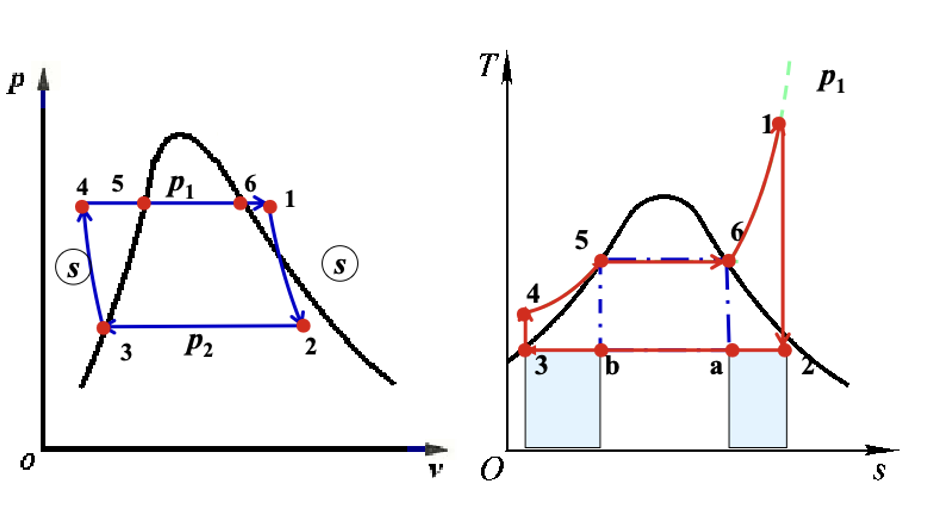
\includegraphics[width=\linewidth]{figures/10朗肯循环.png}
\end{minipage}

\pt{能量关系}：
\begin{itemize}
    \item $w_{t,T}=h_1-h_2$，$w_{t,P}=h_4-h_3$
    \item $q_1=h_1-h_4$，$q_2=h_2-h_3$
    \item $w_{\mathrm{net}}=(h_1-h_2)-(h_4-h_3)$。
\end{itemize}

\pt{朗肯循环热效率}：$\eta_{\mathrm{t}}=\frac{w_{\mathrm{net}}}{q_1}=\frac{(h_1-h_2)-(h_4-h_3)}{h_1-h_4}=1-\frac{h_2-h_3}{h_1-h_4}$。因 $w_{t,P}\ll w_{t,T}$，常取 $h_4\approx h_3$，$\eta_{\mathrm{t}}\approx\frac{h_1-h_2}{h_1-h_3}$，$w_\mathrm{net}\approx w_{t,T}$。

\pt{耗汽率}：装置每输出单位功量所消耗的蒸汽量。\pt{理想耗汽率} $d_0=\frac{1}{h_1-h_2}$；若 $h$ 用 $\mathrm{kJ/kg}$、功用 $\mathrm{kW\cdot h}$，$d_0=\frac{3600}{h_1-h_2}\,\mathrm{kg/(kW\cdot h)}$。耗汽量 $D_0=d_0P_0$。

\divider

\pt{提高初温 $T_1$}：平均吸热温度 $\bar T_1\uparrow$，$\bar T_2$ 不变，$\eta_{\mathrm{t}}\uparrow$，且末端干度 $x_2\uparrow$；受材料耐温限制。

\pt{提高初压力 $p_1$}：平均吸热温度 $\bar T_1\uparrow$，$\bar T_2$ 不变，$\eta_{\mathrm{t}}\uparrow$，但末端干度 $x_2\downarrow$，$p$ 过高，设备强度要求提高。

\pt{降低背压 $p_2$}：$\bar T_1$ 基本不变，平均放热温度 $\bar T_2\downarrow$，$\eta_{\mathrm{t}}\uparrow$，但受环境温度、冷却水温限制，不能随意降低，且 $x_2\downarrow$。

\divider

\noindent
\begin{minipage}
    [t]{0.64\linewidth}
    \vspace{0pt}
    \raggedright
    \pt{有摩阻实际朗肯循环}\\
    实际汽轮机膨胀存在摩阻和不可逆损失：
    \begin{itemize}
        \item 理想膨胀终点为 $2$，实际膨胀终点为 $2_\mathrm{act}$。
        \item 实际过程熵增大，$T-s$ 图上 $2_\mathrm{act}$ 通常位于理想等熵终点 $2$ 的右侧。
    \end{itemize}
\end{minipage}
\hfill
\begin{minipage}
    [t]{0.35\linewidth}
    \vspace{0pt}
    \centering
    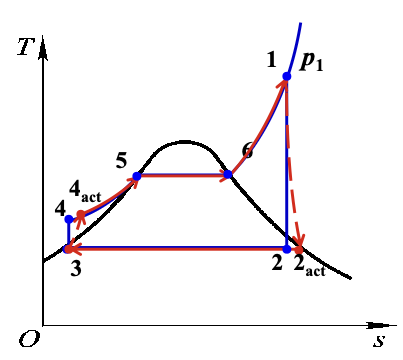
\includegraphics[width=\linewidth]{figures/10实际朗肯循环.png}
\end{minipage}

放热量增大、做功减少、效率下降。汽轮机相对内效率（汽机效率）
$\eta_T=\frac{h_1-h_{2\mathrm{act}}}{h_1-h_{2}}\approx 0.92$（近代大功率汽轮机）。

确定 $h_{2,\mathrm{act}}$ ：\pt{运行中}：测出 $p_2$ 和 $x_2$，用 $h_x=x_2h''+(1-x_2)h'$ 求湿蒸汽焓；\pt{设计中}：选定 $\eta_T$，用 $h_{2,\mathrm{act}}=h_1-\eta_T(h_1-h_2)=h_2+(1-\eta_T)(h_1-h_2)$。

$h_1-h_2$ 称为理想绝热焓降。

忽略泵功时，装置内部热效率 $\eta_i\approx\eta_T\eta_{\mathrm{t}}$；考虑机械效率 $\eta_m$ 时，有效热效率 $\eta_e=\frac{P_\mathrm{e}}{q_1}=\eta_T\eta_m\eta_{\mathrm{t}}$。实际内部耗汽率 $d_i=\frac{d_0}{\eta_T}$，耗气量 $D_i=d_iP_i$，$P_i$ 为实际内部功率。

\divider

\noindent
\begin{minipage}
    [t]{0.64\linewidth}
    \vspace{0pt}
    \raggedright
    \pt{再热循环}

    蒸汽由 $1$ 在高压汽轮机膨胀到 $b$，回锅炉再热到 $a$，再进低压汽轮机膨胀到 $2$。

    忽略泵功时，$w_{\mathrm{net}}=(h_1-h_b)+(h_a-h_2)$，$q_1=(h_1-h_3)+(h_a-h_b)$，$\eta_{\mathrm{t}}=\frac{h_1-h_b+h_a-h_2}{h_1-h_3+h_a-h_b}$。与再热压力有关
\end{minipage}
\hfill
\begin{minipage}
    [t]{0.35\linewidth}
    \vspace{0pt}
    \centering
    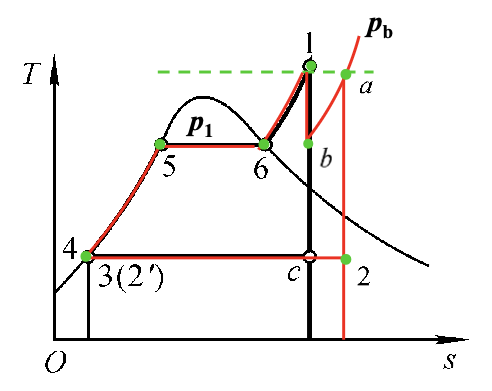
\includegraphics[width=\linewidth]{figures/10再热循环.png}
\end{minipage}

\pt{再热作用}：根本目的是提高汽轮机排汽干度；可降低耗汽率，但是会使得系统复杂
\begin{itemize}
    \item 再热压力过低时，与原循环相比，$T_{m2}$ 不变，$T_{m1}$ 下降，$\eta_\mathrm{t}$ 下降。
    \item 再热压力过高时，与原循环相比，$T_{m2}$ 不变，$T_{m1}$ 上升，$\eta_\mathrm{t}$ 上升，但 $x_2$ 改善不大。
\end{itemize}

\divider

冷凝器出来的温度过低，没有利用价值，因此不能像燃气轮机一样回热

\tdo{对不起这一块看不懂}

\pt{抽汽回热}：从汽轮机中间级抽出部分蒸汽加热给水，提高锅炉入口给水温度，减少低温段外部吸热。方式有混合式和间壁式。

\begin{center}
    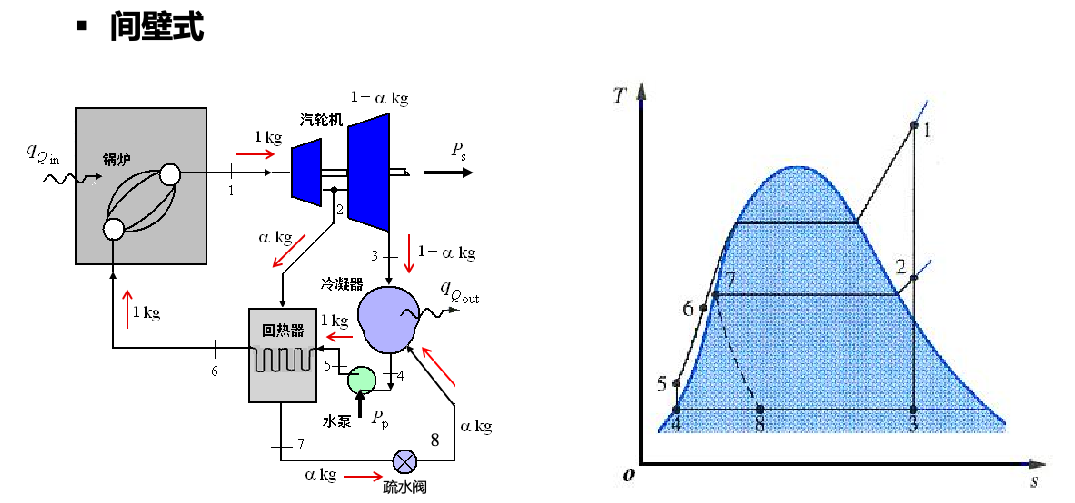
\includegraphics[width=\linewidth]{figures/10间壁式回热.png}\\
    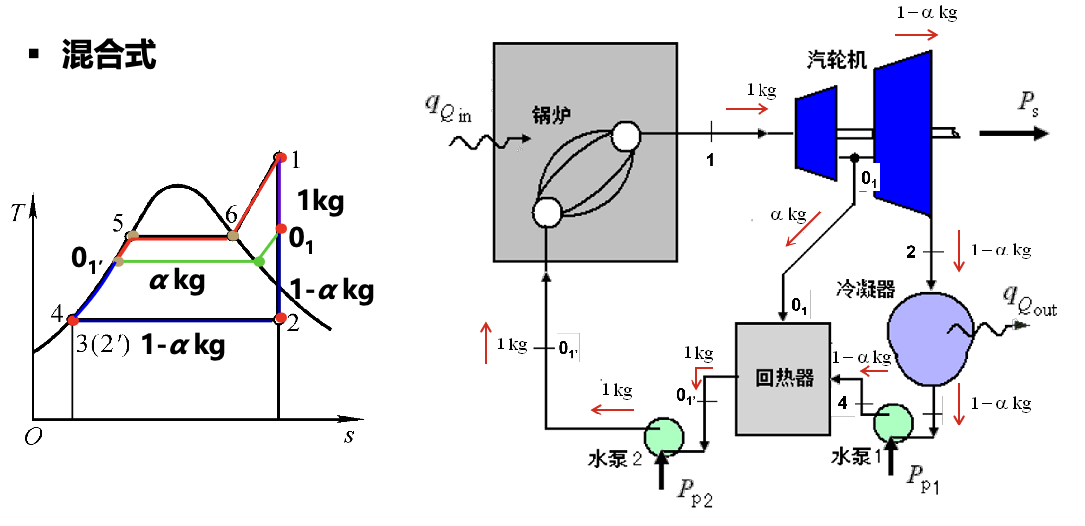
\includegraphics[width=\linewidth]{figures/10混合式回热}
\end{center}

\pt{混合式抽汽量}：主蒸汽取 $1\,\mathrm{kg}$，抽汽量 $\alpha$

抽汽量计算：
\begin{itemize}
    \item 回热器能量方程为 $(1-\alpha)h_4+\alpha h_{01}-h_{01'}=0$。
    \item 忽略泵功时，$h_4 \approx h_{2'}$。
    \item 抽汽系数为 $\alpha=\dfrac{h_{01'}-h_{2'}}{h_{01}-h_{2'}}$。
\end{itemize}

回热器不可逆损失：
\begin{itemize}
    \item 回热器熵方程写为 $(1-\alpha)s_{2'}+\alpha s_{01}-s_{01'}+S_f+S_g=\Delta s_{\mathrm{CV}}$。
    \item 稳态时取 $\Delta s_{\mathrm{CV}}=0$。
    \item 熵产为 $S_g=s_{01'}-\alpha s_{01}-(1-\alpha)s_{2'}$。
    \item 损失为 $I=T_0S_g$。
\end{itemize}

回热循环分析（忽略水泵功）：
\begin{itemize}
    \item 净功为 $w_{\mathrm{net}}=(1-\alpha)(h_1-h_2)+\alpha(h_1-h_{01})$。
    \item 也可写为 $w_{\mathrm{net}}=(h_1-h_{01})+(1-\alpha)(h_{01}-h_2)$。
    \item 吸热量为 $q_1=h_1-h_{01'}$。
    \item 放热量为 $q_2=(1-\alpha)(h_2-h_{2'})$。
    \item 热效率为 $\eta_{\mathrm{t}}=\dfrac{w_{\mathrm{net}}}{q_1}=\dfrac{(h_1-h_{01})+(1-\alpha)(h_{01}-h_2)}{h_1-h_{01'}}$。
    \item 也可写为 $\eta_{\mathrm{t}}=1-\dfrac{q_2}{q_1}=1-\dfrac{(1-\alpha)(h_2-h_{2'})}{h_1-h_{01'}}$。
\end{itemize}

回热循环与原循环比较：
\begin{itemize}
    \item 平均放热温度 $T_{m2}$ 不变；
    \item 平均吸热温度 $T_{m1}$ 上升；
    \item 因此热效率 $\eta_{\mathrm{t}}$ 提高；
    \item 回热的本质是减少低温段外部吸热，使锅炉吸热更多发生在较高温度区间。
\end{itemize}

\pt{回热循环}：$w_{\mathrm{net}}=(h_1-h_{01})+(1-\alpha)(h_{01}-h_2)$，$q_1=h_1-h_{01'}$，$q_2=(1-\alpha)(h_2-h_{2'})$。回热器熵产 $S_g=s_{01'}-\alpha s_{01}-(1-\alpha)s_{2'}$，损失 $I=T_0S_g$。

\pt{提高经济性主线}：提高平均吸热温度、降低平均放热温度、减少不可逆。再热偏向改善末级湿度，回热偏向提高平均吸热温度，大型机组常联合采用。

\divider
